\documentclass[letterpaper, 10 pt, conference]{ieeeconf}
\usepackage{fullpage}
\usepackage{amsmath,amsfonts,amssymb}
\usepackage{verbatim}
\usepackage{graphicx}
\usepackage{tabularx}
\usepackage{booktabs}
\usepackage{multirow}
\usepackage{algorithm}
\usepackage{algorithmic}
%\usepackage{algpseudocode}
\usepackage{xargs}
\usepackage{xspace}
\usepackage[hyphens]{url}
\IEEEoverridecommandlockouts
\overrideIEEEmargins
\floatname{algorithm}{Algorithm}
\usepackage[algo2e]{algorithm2e}
\renewcommand{\algorithmicrequire}{\textbf{Input:}}
\renewcommand{\algorithmicensure}{\textbf{Output:}}
\newcommand{\inlinecode}{\texttt}
% Insert comments
%\usepackage[colorinlistoftodos,prependcaption,textsize=tiny]{todonotes}
%\newcommandx{\kasper}[2][1=]{\todo[linecolor=blue,backgroundcolor=blue!25,bordercolor=blue,#1]{Kasper: #2}}
\newcommand{\tool}[0]{\textsc{TOOLNAME}\xspace}
\title{Analysis of Uncertainty Management for Airport Surface Planning}% and Scheduling}
\author{Robert Morris$^{1}$ \and Heron Yang$^{2}$  \and Corina Pasareanu$^{3}$ \\ % <-this % stops a space
\thanks{$^{2}$ Heron Yang {\tt\small heronyang@cmu.edu}} \\
\thanks{$^{1}$ Robert Morris {\tt\small robert.a.morris@nasa.gov}} \\%
\thanks{$^{3}$ Corina Pasareanu {\tt\small corina.pasareanu@west.cmu.edu}}%
}
\begin{document}
\maketitle
\begin{abstract}%planning
Designing efficient and robust automated planning and scheduling systems for complex logistics applications presents many challenges, especially if the executing environment is changing unpredictably.  In this paper, we study the problem of planning and scheduling airport surface movement. We discuss a simulation framework comprised of a generic airport simulation tool that is easily extensible to different scenarios and airports, and is capable of simulating uncertainty in the form of unexpected delays in aircraft movement. We explore different scheduling methods and also created an uncertainty-aware scheduler which produces robust schedules with simulated uncertainty. Lastly, we built an uncertainty module to model real-word uncertainty and evaluate the robustness of scheduler in light of different scenarios. The system developed is open sourced at \url{https://github.com/heronyang/airport-simulation}.
\end{abstract}
\section{Introduction}

Airport surface operations present a difficult, large-scale logistics problem with a wide range of sub-problems requiring multi-criteria optimization, including: runway sequencing and scheduling; spot or gate release scheduling; gate allocation and taxi route planning and scheduling \cite{malik} \cite{Rathinam}, \cite{Ravizza}, \cite{Roling}.

Airport surface movement optimization is NP-hard \cite{Reif}. Several types of constraints are involved, including pushback times, taxiway layouts, and runway and taxiway separation. Surface movement planning and scheduling is dynamic, with aircraft continuously entering and leaving the operating space. Surface movement is unpredictable and prone to unexpected changes in operating conditions due to things like weather. In general, efficiency and safety are difficult objective to achieve in practice, due to the challenges posed by the presence of uncertainties, human factors, and competing stakeholder interests.

Current practice handles the dual problems of complexity and uncertainty in two ways: continuous planning and scheduling and sub-optimal heuristic scheduling \cite{malik}.  Furthermore, virtually all planning and scheduling decisions are currently made by human operators. Typically, airport surveillance data and scheduling tasks (for departures and arrivals) provide inputs to planning and scheduling. To handle the dynamics of the operations, schedules are revised continuously (for example, every 15 minutes at busy airports). Second, the complexities of the planning and scheduling problem have until now forced the utilization of heuristic approaches to optimization that require reduced computational overhead while achieving useful results.

%In this paper we focus on analyzing the relationship between tightness and performance factors of a scheduler: we expect to see that a scheduler with low tightness brings better performance, vice versa. Furthermore, we study how uncertainty affects the decisions made by a scheduler within our simulation environment, based on the data from the San Francisco Airport. We've observed how different amount of uncertainty generates conflicts on an airport surface, and it's planned to implement a scheduler that refers to predictions with uncertainties generated by a simulator while scheduling. We expect to see a relationship between the uncertainty sensitivity and the real performance.

%\section{Problem}
The goals of this paper are as follows:
\begin{itemize}
\item Build simulation models of common uncertainties in airport surfaces;
\item Quantify the performance of systems combining deterministic planners and schedulers with continuous replanning as the means to handle uncertainty; and
\item Investigate the potential for improved performance through the use of predictive models of uncertainty during scheduling.
\end{itemize}
In the next section we describe the model and algorithms used for planning and scheduling. In section three we discuss the simulation system and visualizer. In section four we describe experiments conducted with a deterministic scheduler using the simulator. We conclude with a discussion of future work.
\section{Approach}
%\section{Multi-agent Path Planning}

Using a technique discussed in \cite{flow}, we define a {\em multi-agent path planning problem (MAPPP)}. The first step in this formulation is a transformation of a node-link model into a unit-distance graph $G = \langle V, E \rangle$ comprised of a set of vertices $V$ and a set of edges $E$ representing a unit distance between vertices, i.e., a distance related to discrete time-steps in the execution of a path. To handle holding actions, we assume that each vertex has an edge directed to itself; i.e., $\{ \langle v_i, v_i \rangle \} \in E$ for all $v_i \in V$.

Given a set $A = \{a_1,\ldots,a_k\}$ of agents, and a time horizon $H = 0 \ldots T$, we define the {\em state} of an agent as a triple $\langle a_i, v_j, t_k \rangle$ of agent, vertex in $G$ and time in $H$. An {\em itinerary} $I$ is a set of tuples $\langle a_i, v_{s,i}, v_{g,i}, e_t, d_t \rangle$ consisting of an agent, a start and goal vertex, a time $e_t$ representing the time the agent enters the planning system, and its scheduled arrival or departure time. Given $I$, a {\em feasible path} for an agent $a_i$ is a sequence of vertices $P = \langle v_0, \ldots, v_n \rangle$, where $v_0 = v_{s,i}$, $v_n = v_{e,i}$, and there are edges $\langle v_k, v_{k+1}\rangle \in E$ for $k = 1 \ldots n-1$.  The length of a path is the number of vertices in the path. A {\em route} between two vertices in $G$ is a path with no duplicated vertices.  A feasible path for an agent corresponds to a sequence of states $S_a = [ \langle a, v_j, t_k \rangle]$. We write $P(S_a ) = \langle v_0, \ldots, v_n \rangle$ to represent the path defined by the sequence of vertices in $S_a$.

An {\em action model} defines the allowable transitions between states, i.e. a set of actions $A_i : S \rightarrow S'$, where $A_i(S) = S'$. The action model used here consists of two actions: $hold$ and $move$, defined by $hold(\langle a_i, v_j, t_k \rangle) = \langle a_i, v_j, t_{k+1} \rangle$ and $move(\langle a_i, v_j, t_k \rangle) = \langle a_i, v_l, t_{k+1} \rangle$, where $\langle v_j, v_l \rangle \in E \footnote{Of course, if there are multiple vertices to which an agent can move, an argument should be added to $move$ to distinguish among the different destinations. But as we'll see later, for this MAPPP this argument won't be required.}$. A feasible transition sequence is a sequence $TS = S_0, A_0, S_1, A_1, \ldots A_n, S_n$, where $P(S_0, \ldots S_n)$ is a feasible path, and $A_i(S_i) = S_{i+1}$ for all $i = 0, \ldots n-1$. $S_0$ ($S_n$) will be called the initial (terminal) state. Similarly, given an initial state $S_s$ and goal state $S_g$, a {\em plan} is a sequence of actions $A_0, A_1, \ldots A_n$ such that $S_s, A_0, S_1, A_1, \ldots A_n, S_g$  is a feasible transition sequence from the start to goal states. The action model $M = \{ hold, move\}$ is used by the planner to generate a plan sequence. Notice that if a path is a route, a corresponding transition sequence has the form $S_0, move, S_1, move, \ldots, move,  S_n$. This special case will be called the {\em unimpeded} transition sequence, with associated unimpeded plan abbreviated by $move_{0, \ldots n-1}$. Thus, without fear of ambiguity, we use feasibility interchangeably to define paths, state sequences and transition sequences.

In addition, because we are solving a continuous planning problem, we extend the action model to include actions not assigned by the planner; specifically we define two actions $exit, enter$ that define when an agent enters or exits the planning problem. The passing of time and the itinerary $I$ determine when an agent enters the system: specifically given $\langle a_i, v_{s,i}, v_{g,i}, e_t, d_t \rangle \in I$, agent $a_i$ enters the problem at time $e_t$. Conversely, given a transition sequence with terminal state $S_n = \langle a, v_j, t_k \rangle$, agent $a$ leaves the problem at time $t_{k+1}$.  Finally, we say an agent is {\em active} if it  entered the problem but has not exited.

Given two transition sequences $TS_{a_0}, TS_{a_1}$  a {\em conflict} is a pair of states $\langle a_0, v_j, t_k \rangle \in TS_{a_0}, \langle a_1, v_j, t_k \rangle \in TS_{a_1}$. There are two kinds of conflict: a move-move conflict is the result of two (or more) agents converging to a single vertex; a move-hold conflict is the result of one agents moving to a vertex in which another is holding. All conflicts are resolved by introducing delays (hold actions) on agent plans. Resolving either kind of conflict might result in the creation of one or more new move-hold or move-move conflicts. The total number of hold insertions needed to create a conflict-free feasible set of transition sequences is bounded by the number of agents, as well as the length of the longest route between start and goal states.

A MAPPP is a tuple $\langle G, I, A \rangle$, where $G$ is a unit-distance graph, $I$ an itinerary, and $A$ a set of agents. A solution to a MAPPP is a collection of conflict-free feasible Transition Sequences $TS = \{TS_{a_1}, \ldots, TS_{a_n}\}$ for each $a_i \in A$. Solving an MAPPP consists of finding a path plan for each agent: a sequence of actions that defines a feasible transition sequence from a start state to a goal state that does not contain states that conflict with states of other agents.
\subsection{Planning Approach}

The interest here is in representing the airport surface scheduling problem by casting it as a MAPPP, where the agents are aircraft arriving or departing. Drawing upon previous work on solving the same problem, and on characteristics of real airport operations, we first make the simplifying assumption that given a start and goal vertex $v_s, v_g$, e.g. corresponding to a gate and runway node for departing aircraft, there is a single predetermined route $R_{v_s, v_g}$ assigned to any aircraft. This simplifies the problem while making it more realistic for airport surface planning, but the assumption can be removed without fundamentally changing the overall approach adopted here.

The second characteristic of airport surface planning is uncertainty. Specifically, a solution to a MAPPP may lead to conflicts when executed, due to unexpected delays. In general, there are two ways to handle uncertainty: by anticipating them at planning time by applying uncertainty models, or by responding to unanticipated changes to the operational environment by continuous re-planning. The interest of the research effort here is in both approaches to handling uncertainty.

First, we define an approach to continuous re-planning based on the idea of a {\em rolling horizon} (RH) \cite{clare}.   The RH variable defines a moving window for solving a subproblem of the complete planning problem. Given a  rolling horizon of N, the inputs to a RH planner is a set of current states $\{\langle a_i, v_j, t_k \rangle\}$ for each $a_i$ in the set of active aircraft. The output of the planner is a set of feasible conflict-free transition sequences of the form $\langle a_i, v_j, t_k \rangle, A_k, \langle a_i, v_{j+1}, t_{k+1}\rangle A_{k+1}, \ldots ,  A_{k+N}, \\ \langle a_i, v_{j+N}, t_{k+N} \rangle$. For uniformity, if an aircraft enters or exits the plan within the planning horizon, the states and actions before entering or after exiting consist are designated as NULL actions and NULL states.

In an environment with no delay uncertainty, the result of executing any RH-plan $P =A_{k, \ldots,  k+N}$ from a set of initial states of the form $\{\langle a_i, v_j, t_k \rangle\}$ would be a set of states $S_{rh} = \{ \langle a_i, v_{j+N}, t_{k+N} \rangle \}$ for each $a_i \in A$. Equivalently, the degree of delay uncertainty determines the extent to which the the set of states $S$ resulting from executing $P$ from the set of initial states differs from $S_{rh}$. To avoid conflicts from unexpected delays, we introduce a re-planning variable RP that designates the time between RH-planning, thus controlling the effects of uncertainty. Specifically, a smaller RP allows for more frequent sampling of the current active states, thus allowing for adjustment to unexpected delays in the execution of plans.
\begin{algorithm}[H]
\caption{RH Planner}
\SetAlgoLined
{\bf Inputs}: Initial states $S = \{ \langle a_i, v_j, t_K \rangle \}$; Itinerary $I$;  Routes $ \{ R_i = v_0 \ldots v_M\}$ for all $a_i$ in the set of active aircraft; A Rolling Horizon $N$ \\
{\bf Output}: A set of conflict-free feasible Transition Sequences $TS$ and associated plans $A$ for each initial state in $S$
\begin{enumerate}
\item Form the set $TS_u$ from generating the unimpeded transition sequence $S_j, move, S_{j+1} \ldots , move, S_{j+N}$ for each initial condition $S_j = \langle a_i, v_j, t_K \rangle \in S$, where $P(S_j, \ldots, S_{j+N}) = v_j, \ldots v_{j+N}$ taken from $R_i$, the preassigned route for $a_i$.
\item Initialize the set $C$ of conflicts in $TS_u$
\item Let $TS_u$ and $C$ provide the seed to local search to find a conflict-free feasible transition sequence $TS$
\item return $TS$
\end{enumerate}
\label{rh}
\end{algorithm}

The RH-planner pseudo-code is found in Figure~\ref{rh}. There are three main computational components of the RH-planner: first, generating the initial unimpeded transition sequences, one for each initial state in the input of states ($O(N)$, step 1); second, detecting the set of conflicts in a set of transition sequences ($O(N^2)$, steps 2 and 3); finally, in the application of local search to repair a conflicted set of transition sequences.

\subsubsection{Local Search for Conflict Resolution}

\section{Simulation System}

The Airport Surface Simulation and Evaluation Tool, ASSET2, is designed and developed to evaluate our proposed planner under uncertainties. ASSET2 is a generic tools for research purpose as it supports surface data of different airports and runs simulations based on customized experiment plans.

\subsection{Components}

In ASSET2, {\it Simulator} configures the experimental parameters and initializes one or many simulations. {\it Simulation}, a callee of the {\it Simulator}, is a conductor which manipulates an airport surface movement of a day by applying itineraries generated by the RH-planner.

Within {\it Simulation}, there are static objects containing immutable data of the simulation, dynamic objects representing run-time states, and the stateless object for computations, the scheduler. Examples of static objects are {\it Surface}, {\it Scenario} and {\it Routing Table}; and dynamic object examples are {\it Airport} (contains a list of {\it Aircraft}) and {\it Clock}. A detailed description of the above objects is included in Table \ref{simulation-objects}.

\begin{table}[htbp]
\centering
\begin{tabularx}{\linewidth}{
    |>{\hsize=.15\hsize}X
    |>{\hsize=.85\hsize}X|}
\hline
 & {\bf Description} \\ \hline
{\it Surface} & Contains airport surface data of the gates, spot positions, taxiway, runway, etc. \\ \hline
{\it Scenario} & Contains a list of departure and arrival flight information include their designated gates and runways. \\ \hline
{\it Routing Table} & Used by {\it Routing Expert} object for giving the shortest route between two nodes. \\ \hline
{\it Airport} & Contains a list of active aircrafts, queues at gates, and the {\it Surface} object \\ \hline
{\it Clock} &  Contains the simulated time of a day. \\ \hline
{\it Scheduler}  & Generates itineraries per active aircraft every reschedule cycle. \\ \hline
\end{tabularx}
\label{simulation-objects}
\caption{Description of objects in {\it Simulation}}
\end{table}

An unit-distance link-node model is applied as a foundation of all objects on the surface. Gates, spot positions, are locations of aircrafts are inherited from a {\it Node} object while runways, taxiways, etc, are inherited from a {\it Link} object.

\subsection{Flow}

\subsubsection{Data Preparation}

Two kinds of data are required for executing a simulation, the airport surface data and the scenario data. For the airport surface data, it is usually be presented in a KML file format, and that can be parsed into several JSON files by our script and be used as an input for the simulation. A complete surface data of an airport include the name and geolocation of the gates, spot positions, taxiways, push-back ways, and the runways. For scenario data, they are randomly generated per simulation \footnote{The scenario data can also be provided and be parsed into the format recognized by the simulation in the case of testing real-world scenarios.}. The time gap between two generated flights is based on a normal distribution value while the mean and the deviation value are given.

\subsubsection{Initialization}

To execute a simulation, an {\it experimental plan} describing a set of the configurations is given. {\it Simulation} loads data from the file specified in the {\it experimental plan} then discretizes the links. {\it Routing Expert} object then calculates the shortest path between any two nodes using the Floyd Warshall algorithm and caches the routing table for future usages.

\subsubsection{Simulation}

Within a simulation, we keep a virtual time, $t_v$, in {\it Clock} representing the time of the day and define a constant time value $T_S$ as the simulation time unit. The {\it Simulation} only simulates the states at $t_v = n * T_S, n = 0, 1, ...$; therefore, $T_S$ is similar to the resolution of the simulation.

For objects containing run-time states, the \inlinecode{tick()} function is implemented to update the states of $t_v$ to $t_v + T_S$. {\it Simulation} calls its own \inlinecode{tick()} function in a loop until {\it Clock} object reports the simulated day has reached the end. Inside the \inlinecode{tick()} function, {\it Simulation} first checks if it's a time to reschedule, and if yes, it passes the delegate of the simulation to {\it Scheduler} and retrieve a list of itineraries for each active aircrafts. After applying the itineraries on the aircrafts, it injects uncertainty delays, adds new aircrafts according the {\it Scenario} object, calls the \inlinecode{tick()} function of the {\it Clock} object and all the active aircrafts. Eventually, after the loop is finished, {\it Simulation} asks the {\it State Logger} object and the {\it Analyst} object to save the output metrics into files or plots. A detailed sequence diagram is shown in Fig. \ref{flow}.


% Source: https://www.draw.io/#G1IZkLn2qqXytbG_RAj9IK3dkFLM4_dIqh

\begin{figure*}[h]
\caption{Sequence diagram of the tick() function}
\centering
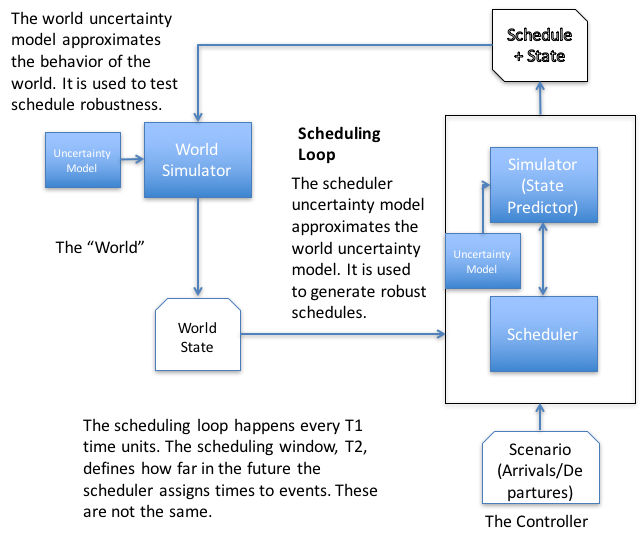
\includegraphics[width=\textwidth]{flow}
\label{flow}
\end{figure*}

\subsubsection{Scheduler}

{\it Scheduler} is stateless and is called by {\it Simulation} once very reschedule cycle. It offers a function, \inlinecode{schedule(simulation) => itineraries)}, that reads the current simulation state and returns a list of itineraries for each active aircraft. {\it Scheduler} is able to use the run-time states within the simulation object to make scheduling decisions, or to make a copy of the simulation and predict the future states by calling the \inlinecode{tick()} function of the cloned simulation object.

\subsubsection{Visualization}

A web-based visualization tool is provided for viewing a simulation result or for debugging. The tool reads the output metrics of a single simulation, and plot them onto the web interface using Google Map API.

\subsubsection{Batch Execution}

Batch execution of the simulations are developed and used for running the same simulation for multiple times with or without different experimental values. To implement this feature, {\it Simulator} first decides how many runs are asked and what parameter to change per run by reading the given experimental plan. Then, {\it Simulator} execution single simulations one by one. Last, {\it Simulator} reports the accumulated output metrics into another set of output files.

\section{Experiments}

\subsection{Dataset}

To evaluate our purposed model under a real-world environment and to avoid starting with an over-complex dataset, we picked partial San Francisco International Airport, Terminal 2, as our dataset. In this surface data, there are 14 gates, two spot positions, 14 push-back ways, 25 taxiways, and 1 runway (see Figure \ref{sfo-terminal-2}). Before each simulation, the scenario data is randomly generated where the time gap between two aircrafts is a Gaussian random number with a mean value 300 seconds and a deviation 60 seconds.

% FIXME: How to reference the SFO data source? It is based on the Open-Street dataset from last semester and the inventory PDF file.

\begin{figure}[h]
\caption{Surface Data of Terminal 2, San Francisco International Airport}
\centering
\includegraphics[width=0.5\textwidth]{sfo-terminal-2}
\label{sfo-terminal-2}
\end{figure}

\subsection{Environment Setup}

\subsubsection{Control Variables}

Two major control variables are selected based on the computation capacity of our machine. First, we selected 30 seconds as {\it the time unit of our simulation}  representing the virtual time passed by per \inlinecode{tick()}. Second, we selected 5 as the number of simulation samples we execute per one experiment setting and the average of the output metrics is used as our final output metrics.

% NOTE: if we change the *simulation time unit*, and *the number of samples* later, we should change the numbers here as well.

\subsubsection{Experimental Variables}

We define the {\it reschedule time cycle} as the time period between two schedule action done by the scheduler, and the {\it uncertainty amount} as the possibility of a single-tick delay injected to the aircraft at a gate per \inlinecode{tick()}. We launch two batch executions for testing different {\it reschedule time cycle} and different {\it uncertainty amount} injected while other variables are given.

\subsubsection{Output Metrics}

For each simulation, we collect several output metrics including the number of delays injected by the uncertainty model and the schedule, the queue size at the gate, the execute time of rescheduling, and the failure rate. The details of each metric is described below in Table \ref{output-metrics}.

\begin{table}[htbp]
\centering
\begin{tabularx}{\linewidth}{
    |>{\hsize=.30\hsize}X
    |>{\hsize=.70\hsize}X|}
\hline
 & {\bf Description} \\ \hline
{\it Number of delay injected} & Per \inlinecode{tick()}, we count the number of aircrafts delayed by the uncertainty model or the scheduler. \\ \hline
{\it Queue size at gate} & The later flights are be added into a queue at the gate if the gate is occupied by a previous flight. Per \inlinecode{tick()}, we log the total size of the queues at gate. \\ \hline
{\it Reschedule execution time} & Per reschedule done by the scheduler, we log the actual time it take in the unit of seconds. \\ \hline
{\it Failure rate} & If a conflict occurs, we abort the whole simulation and count it as a failure simulation run. The failure rate is calculated by the number of failures divided by the total number of simulation runs. \\ \hline
\end{tabularx}
\label{output-metrics}
\caption{Description of the output metrics}
\end{table}

\subsection{Uncertainty Experiments}

\subsection{Reschedule Time Experiments}

\subsection{Execution Cost}

1. how long it takes for above experiments, and compare between the schedulers

2. how long it takes for running on different size of dataset

\section{Related Work}

\section{Conclusion and Future Work}

%\section{Summary}
\bibliographystyle{IEEEtran}
\bibliography{SFOScheduling}
\end{document}
